\documentclass{article}
\usepackage[left=2.5cm, right=2.5cm, top=2.5cm, bottom=2.5cm]{geometry}
\usepackage{siunitx}
\usepackage{tikz}
\usepackage{pgfplots}
\usepgfplotslibrary{fillbetween}


\begin{document}

\section{2D-Graphs}

\subsection*{2D Grafik}
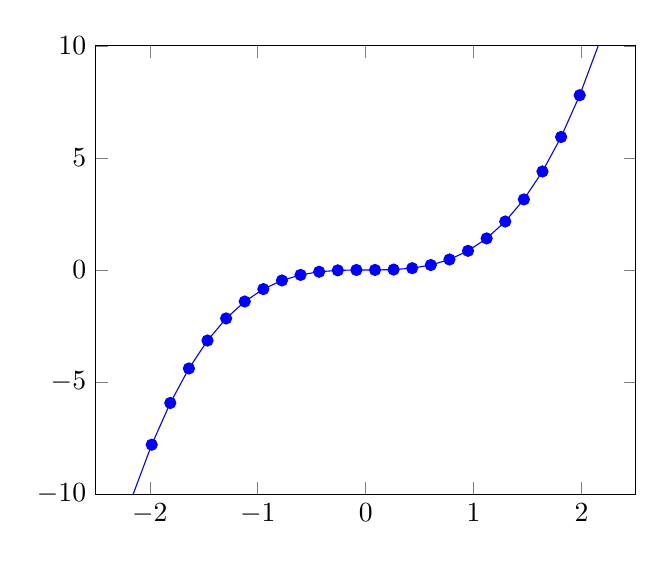
\begin{tikzpicture}[scale=1]
 \begin{axis}[xmin=-2.5, xmax=2.5,ymin=-10, ymax=10]
 	\addplot[color=blue, mark=*, samples=30, domain=-2.5:2.5]{x^3};
 \end{axis}
\end{tikzpicture}

\subsection*{Mit x-Achsen Ticks}
\begin{tikzpicture}
	\begin{axis}[
	clip=false,
	xmin=0, xmax=2*pi,
	ymin=-1, ymax=1,
	axis lines=middle,
	xtick={0, pi/2, pi, 1.5*pi, 2*pi},
	xticklabels={$0$, $\frac{\pi}{2}$, $\pi$,$\frac{3}{2}\pi$, $2\pi$},
	xticklabel style={anchor=south west},
	xmajorgrids=true,
	grid style=dashed]
	\addplot[domain=0:2*pi, red, samples=40]{sin (deg(x))}
	node[right, pos=0.95]{$f(x)=\sin (x)$};
	\end{axis}
\end{tikzpicture}



\subsection*{Mit Koordinaten Punkte}

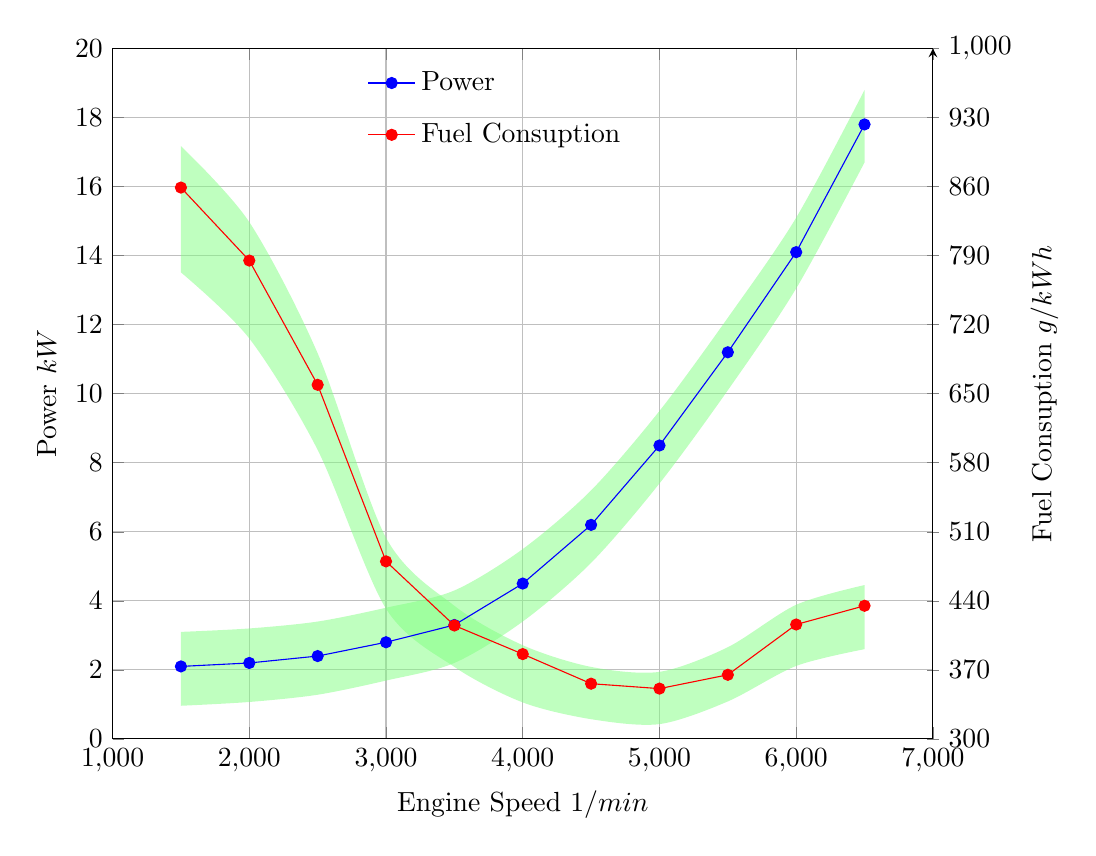
\begin{tikzpicture}
\begin{axis}[
	width = 12cm,
	ymin=0, ymax=20,
	legend style={
	legend style={fill=none},
	draw=none,
	at={(0.3, 0.95)},
	anchor=west},
	axis y line*=left,
	xlabel=Engine Speed $1/min$,
	ylabel=Power $kW$,
	ytick={0,2,...,20},
	xmajorgrids=true,
	ymajorgrids=true]
\addplot[blue, mark=*] coordinates {
(1500,2.1)
(2000,2.2)
(2500,2.4)
(3000,2.8)
(3500,3.3)
(4000,4.5)
(4500,6.2)
(5000,8.5)
(5500,11.2)
(6000,14.1)
(6500,17.8)
};
\addlegendentry{Power}
\addplot+[name path=A, smooth, opacity=0, mark=none] coordinates {
(1500,0.96)
(2000,1.07)
(2500,1.28)
(3000,1.69)
(3500,2.2)
(4000,3.4)
(4500,5.1)
(5000,7.4)
(5500,10.1)
(6000,13.05)
(6500,16.7)
};
\addplot+[name path=B, smooth, opacity=0, mark=none] coordinates {
(1500,3.1)
(2000,3.2)
(2500,3.4)
(3000,3.8)
(3500,4.3)
(4000,5.5)
(4500,7.2)
(5000,9.5)
(5500,12.2)
(6000,15.1)
(6500,18.8)
};
\addplot[green!50, opacity=0.5] fill between[of=A and B];
\end{axis}

\begin{axis}[
	width = 12cm,
	ymin=300, ymax=1000,
	legend style={
	legend style={fill=none},
	draw=none,
	at={(0.3,0.875)},
	anchor=west},
	axis y line=right,
	axis x line=none,
	ylabel=Fuel Consuption $g/kWh$,
	ytick={300,370,...,1000}]
\addplot[red, mark=*] coordinates {
(1500,859)
(2000,785)
(2500,659)
(3000,480)
(3500,415)
(4000,386)
(4500,356)
(5000,351)
(5500,365)
(6000,416)
(6500,435)
};
\addlegendentry{Fuel Consuption}
\addplot+[name path=A, smooth, opacity=0, mark=none] coordinates {
(1500,773)
(2000,706)
(2500,593)
(3000,432)
(3500,373)
(4000,337)
(4500,320)
(5000,315)
(5500,338)
(6000,374)
(6500,391)
};
\addplot+[name path=B, smooth, opacity=0, mark=none] coordinates {
(1500,901)
(2000,824)
(2500,691)
(3000,504)
(3500,435)
(4000,395)
(4500,373)
(5000,368)
(5500,393)
(6000,436)
(6500,456)
};
\addplot[green!50, opacity=0.5] fill between[of=A and B];
\end{axis}
\end{tikzpicture}


\section{3D Plots}

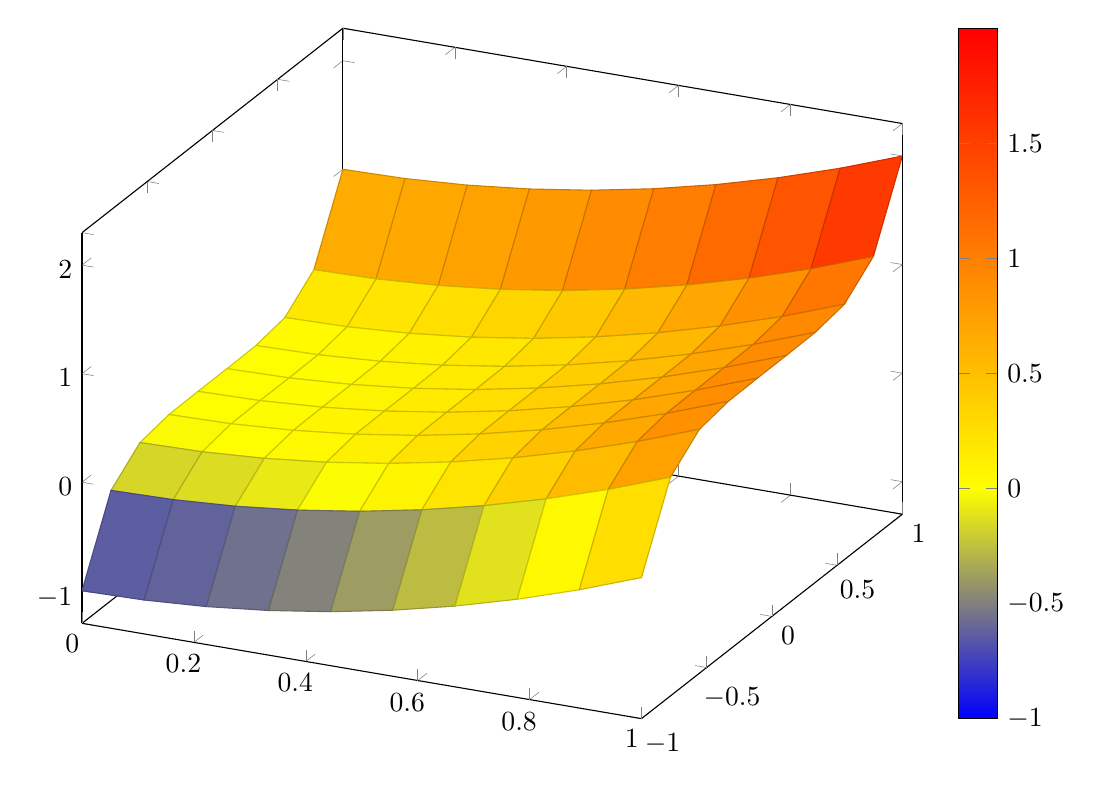
\begin{tikzpicture}
\begin{axis}[colorbar, width=12cm]
\addplot3
[surf,
samples=10,
domain=0:1,y domain=-1:1]
{x^2 + y^5};
\end{axis}
\end{tikzpicture}

\end{document}
